\documentclass[a4paper,norsk,12pt]{article}

\usepackage[norsk]{babel}
\usepackage{enumitem}
\usepackage{color}
\usepackage{amsmath}
\usepackage{wrapfig}
\usepackage{graphicx}
\usepackage[utf8]{inputenc}
\def\d{\ensuremath{\text{d}}}
\def\half{\ensuremath{\frac{1}{2}}}

\begin{document}
Generell prat om hvordan termodynamikk gjør at vi kan håndtere mangepartikkelsystemer uten å trenge informasjon om den mikroskopiske tilstanden.

\chapter{Kinetisk gassteori}
Her beskriver vi hvordan vi kan forstå makroskopiske størrelser som temperatur, varmekapasitet og trykk i gasser som et resultat av summen av bevegelsene til alle atomene i gassen. I mesteparten av kapittelet vil vi kun diskutere ideelle gass, det vil si en hypotetisk gass der
\begin{itemize}
	\item
	gassmolekylene ikke tar opp noe volum,
	\item
	kollisjon mellom gassmolekyler er perfekt elastisk,
	\item
	all indre energi er i form av translasjon\footnote{Dette forutsetter at gassen er  monoatomisk eller at temperaturen er tilstrekkelig lav. Vi skal likevel etterhvert i noen tilfeller også behandle gasser med fleratomige molekyler som om de var ideelle.}, dvs $U = \half mv^2$.
\end{itemize}
Selv om ideell gass er et hypotetisk konsept er dette en god tilnærming for mange reelle gasser. Derfor er ikke en rent teoretisk disuksjon, men også av praktisk nytte.

I avsnitt \ref{sec:kinetiskgassteori:reellgass} kommer en kort beskrivelse av hvordan resultatene i dette kapittelet må modifiseres for reelle gasser der ideell gass-tilnærmingen ikke er tilfredsstillende.

\section{Temperatur}
\label{sec:kinetiskgassteori:temperatur}
Fundamentalt sett er temperaturen til et system et mål på hvor mye energi som er lagret i det. I et fast stoff er energien lagret i form av at atomene vibrerer omkring sin likevektsposisjon, samt i form av bevegelsen til ledningeselektronene hvis det faste stoffet er et metall. Vi skal se mer på faste stoffer i avsnittet om varmekapasitet. I fluider er energien lagret i form av kinetisk energi knyttet til translasjon, rotasjon og vibrasjon. 

Vi begynner med å se på mono	-atomiske gasser, som for eksempel helium. Siden det ikke er noen binding mellom atomer her er det ikke noen 
''fjær'' som kan lagre energi i form av vibrasjon. Vi skal ikke komme videre inn på dette her, men kvantemekanikken forteller oss at en-atomige gasser heller ikke kan lagre energi i form av rotasjon. Dermed er all energi lagret i form av translasjon, slik at den totale energien til gassen kan skrives som
\begin{displaymath}
	E = \sum_i \half mv_i^2
\end{displaymath}
der vi summerer over alle molekylene i gassen.

For at det skal være meningsfullt å snakke om temperatur må systemet være i termodynamisk likevekt\footnote{Strengt tatt er det tilstrekkelig med en lokal likevekt, slik at vi kan tillate en temperaturgradient gjennom gassen. For enkelhets skyld skal vi anta at hele systemet vi ser på er i likevekt.}. Naivt sett skulle man da forvente at hvert atom i gjennomsnitt har den samme energien, men dette viser seg å være feil. I appendiks \ref{apx:maxwellfordeling} viser vi at når en mono-atomisk gass er i likevekt har atomene en hastighet som beskrives av Maxwell-fordelingen,
\begin{equation}
\label{eq:kinetiskgassteori:fv}	
	f(v) = 4\pi\left( \frac{m}{2\pi kT} \right)^{3/2} v^2e^{-mv^2/2kT},
\end{equation}
der $m$ er massen hvert atom, $T$ er temperaturen til gassen og $k = 1.38\times10^{-23}~\mathrm{J/K}$ er boltzmann-konstanten. $f(v)$ er sannsynlighetstettheten for farten $v$, det vil si at sannsynligheten for å finne et atom med fart i intervallet $v_1<v<v_2$ er
\begin{displaymath}
	P(v_1 < v < v_2) = \int_{v_1}^{v_2} f(v) \d v.
\end{displaymath}
Figur (\ref{fig:kinetiskgassteori:Maxwelldist}) viser $f(v)$ for heliumgass ved $T=20^\circ\mathrm{C} = 293~\mathrm{K}$ og $T = 1000~\mathrm{K}$. Ved $293~\mathrm{K}$ ser vi at det store flertallet av atomer har en fart omkring $1000~\mathrm{m/s}$, mens en del atomer har vesentlig større fart. Når temperaturen øker til $1000~\mathrm{K}$ ser vi to endringer. For det første ser vi at temperaturen flest atomer har nå har økt til omkring $2000~\mathrm{m/s}$. For det andre ser vi at spredingen i farten til atomene er større, slik at en mindre andel av atomene har den hyppigst forekommende farten.

\begin{figure}[htp]
	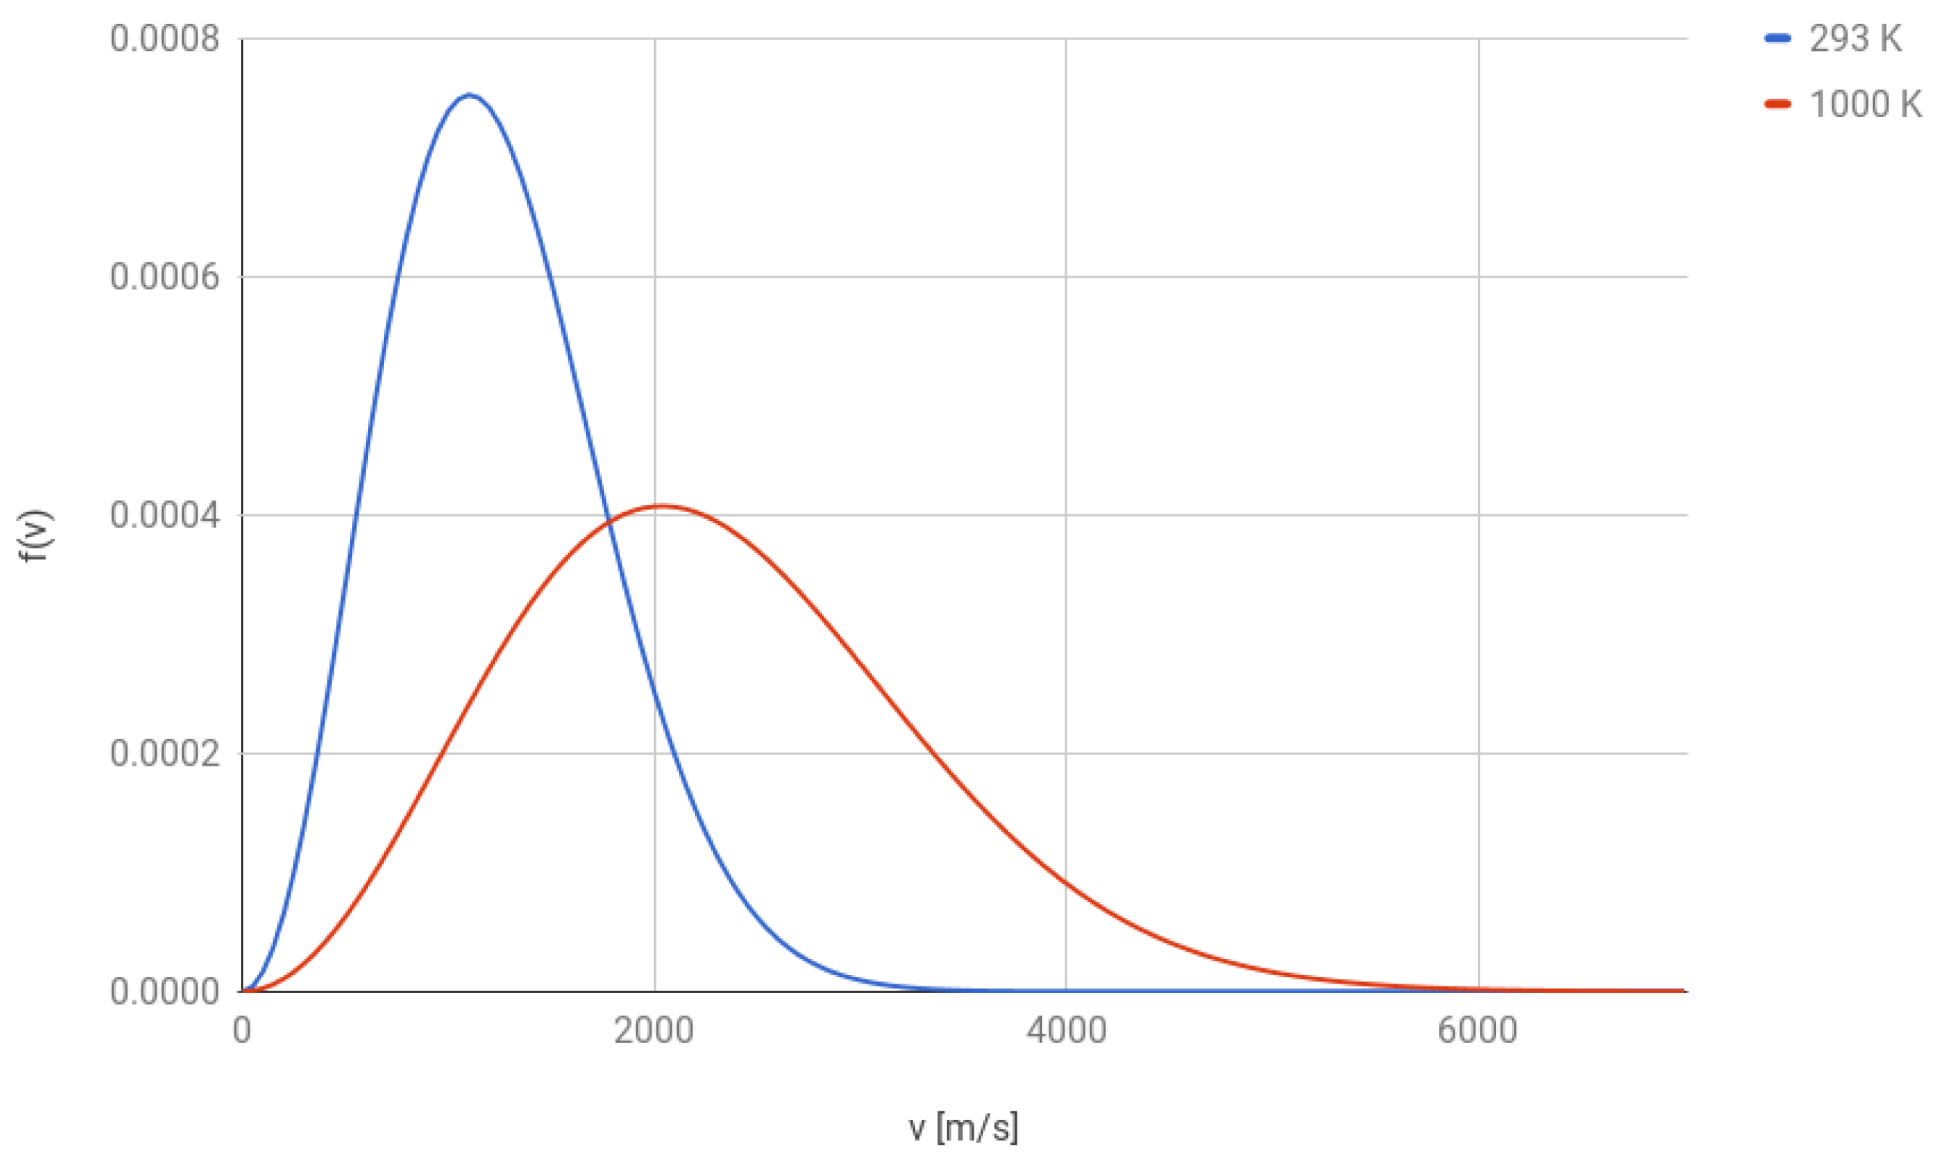
\includegraphics{./MaxwellDistributionHelium}
	\caption{Sannsynlighetsfordeling for farten til atomene i heliumgass ved temperatur 293 K (blå) og 1000 K (rød).}
	\label{fig:kinetiskgassteori:Maxwelldist}
\end{figure}

For å finne den total energien som er lagret i gassen må vi summere over den kinetiske energien til alle enkeltatomene. Siden vi så langt har antatt at alle atomene har den samme massen gir dette ganske enkelt\footnote{Når vi omtaler energien i gassen som helhet bruker vi symbolet $U$ i stedet for $E$ siden det er det vanligste symbolet brukt på indre energi i litteraturen.}
\begin{equation}
\label{eq:kinetiskgassteori:U}
	U = N\frac{1}{2}m\langle v^2 \rangle
\end{equation}
Der $N$ er antall atomer i gassen og $\langle v^2 \rangle$ er middelverdien av $v^2$. Merk forøvrig at $\langle v^2 \rangle \neq \langle v \rangle^2$ siden fartsfordelingen ikke er symmetrisk om den mest sannsynlige farten. Dette diskuteres mer i appendiks \ref{apx:maxwellfordeling}.

Middelverdien til $v^2$ finner vi fra hastighetsfordelingen (\ref{eq:kinetiskgassteori:fv}) ved å beregne integralet
\begin{displaymath}
\begin{aligned}
	\langle v^2 \rangle &= \int_0^\infty v^2 f(v) \d v \\
	&= \int_0^\infty 4\pi\left(\frac{m}{2\pi kT}\right)^{3/2} v^4 e^{-mv^2/2kT}\d v.
\end{aligned}
\end{displaymath}
Beregningen av dette integralet er vist i avsnitt \ref{apx:maxwellfordeling:middel} og gir resultatet
\begin{displaymath}
	\langle v^2 \rangle = \frac{3kT}{m}.
\end{displaymath}
Innsatt i ligning (\ref{eq:kinetiskgassteori:U}) finner vi da at energien til gassen kan skrives som
\begin{equation}
\label{eq:kinetiskgassteori:Eideellgass}
	U = N\half m\langle v^2 \rangle = \frac{3}{2}NkT
\end{equation}
Ofte måles stoffmengden i mol i stedet for i antall atomer. Et mol er $6.022~\times10^{23}$ atomer. Uttrykt i form av mol er energien til gassen 
\begin{equation}
\label{eq:kinetiskgassteori:EideellgassMol}
	U = \frac{3}{2}nRT
\end{equation}
der $n$ er antall mol i gassen og $R = 8.31~\mathrm{J/(mol\cdot K)}$ er en konstant som er relatert til boltzmann-konstanten $k$, og kalles den universelle gasskonstanten.	

Fra det vi har utledet nå ser vi altså at temperaturen til en mono-atomisk gass er direkte proposjonal til summen av kinetisk energi som alle atomene i gassen har. Vi skal ikke se i detalj på gasser med molekyler som består av flere atomer her, men bare konstantere at den samme relasjonen gjelder der også, altså
\begin{displaymath}
	U = N\half m_{CoM}\langle v^2\rangle = \frac{3}{2}nRT.
\end{displaymath}
Merk at det bare er kinetisk energi knyttet til masse-senterets translasjon som går inn i energi-beregningen her, mens energi knyttet til rotasjon eller intern vibrasjon i molekylene ikke er med.


%Siden det er et enormt stort antall atomer kan vi tilnærme summen med et integral der vi bruker fordelingsfunksjonen (\ref{eq:kinetiskgassteori:fv}) som vektfunksjon for å ta hensyn til hvor stor andel av atomene som har enhver gitt fart,
%\begin{displaymath}
%\begin{aligned}
%	E &= \int_0^\infty N vf(v)mv\d v \\
%	&= \int_0^\infty 4\pi N\left(\frac{m}{2\pi kT}\right)^{3/2} mv^4 e^{-mv^2/2kT} \d v.
%\end{aligned}
%\end{displaymath}
%Her er $N$ antall atomer i gassen vi ser på. Denne faktoren må være med fordi $f(v)$ er normalisert slik at den gjelder per atom.
%
%Før vi forsøker å beregne dette integralet omorganiserer vi faktorene litt og gjør et variabelbytte,
%\begin{displaymath}
%\begin{aligned}
%	E &= \frac{4Nm}{\sqrt{\pi}} \int_0^\infty \left(\frac{mv^2}{2kT}\right)^{3/2} e^{-mv^2/2kT} v\d v \\
%	&= \frac{8NkT}{\sqrt{\pi}} \int_0^\infty \left(\frac{mv^2}{2kT}\right)^{3/2} e^{-mv^2/2kT} \frac{mv \d v}{2kT} \\
%	& = \frac{8NkT}{\sqrt{\pi}} \int_0^\infty y^4 e^{-y^2} \d y,
%\end{aligned}
%\end{displaymath}
%der $y^2 = mv^2/2kT$, og følgelig $y\d y = mv\d v/2kT$. Integralet er her av en klasse som kalles gaussiske integraler og som kan beregnes relativt enkelt. Vi skal ikke gå nærmere inn på hvordan det beregnes her, men bare konstantere at
%\begin{displaymath}
%	\int_{-\infty}^\infty y^4e^{-y^2} \d y = \frac{3}{4}\sqrt{\pi}.
%\end{displaymath}
%Siden integralet vårt kun går fra $0$ til $\infty$, og siden integranden er en jamn funksjon har integralet vårt halve verdien av dette, altså $3\sqrt{\pi}/8$. Vi finner dermed at den totale energien er 
%\begin{displaymath}
%	E = \frac{8NkT}{\sqrt{\pi}}\cdot \frac{3\sqrt{\pi}}{8} = 3NkT
%\end{displaymath}



\section{Trykk}
Trykket i et fluid kan forstås som et resultat av bevegelsesmengden til molekylene\footnote{Fluidet består enten av enkeltatomer eller av atomer satt sammen til molekyler. For enkelhets skyld omtaler vi de bare som molekyler her, men diskusjonen er identisk uansett om gassen består av enkeltatomer eller sammensatte molekyler} i fluidet. For å gjøre dette litt mer konkret studerer vi det  trykket fluidet forårsaker på veggene til en beholder. Vi har sett i avsnitt \ref{sec:kinetiskgassteori:temperatur} at molekylene i fluidet beveger seg tilfeldig rundt med en gitt hastighetsfordeling. Denne tilfeldige bevegelsen vil gi stadige kollisjoner med veggene av beholderen. Hver kollisjon kan sees på som et elastisk støt\footnote{Dette er en liten forenkling, men resultatene vi utleder blir likevel riktig så lenge gassen og beholderen er i termisk likevekt.} der hastighetskomponenten til atomet normalt på veggen beholder størrelsen, mens retningen snues. Komponenten parallelt med veggen endres ikke. Dette er illustrert i figur \ref{fig:kinetiskgassteori:deltaV}. Gitt hastighet før kollisjonen
\begin{displaymath}
	\vec{v}_\text{før} = v_\perp \hat{e}_\perp + v_{||} \hat{e}_{||},
\end{displaymath}
der $ \hat{e}_\perp$ og $\hat{e}_{||}$ er enhetsvektorer henholdsvis normalt på veggen og parallelt med veggen, vil altså farten etter kollisjonen være
\begin{displaymath}
	\vec{v}_\text{etter} = -v_\perp \hat{e}_\perp + v_{||} \hat{e}_{||}.
\end{displaymath}
Siden hastighetskomponenten normalt på veggen endrer fortegn får vi en endring i bevegelsesmengde 
\begin{displaymath}
	\Delta \vec{p} = -2mv_\perp\hat{e}_\perp.
\end{displaymath}
Dette betyr at veggen har virket på atomet med en kraft normalt på veggen. Motkraften til denne kraften er den kraften fra molekylet som forsøker å dytte veggen utover. Siden trykk er kraft normalt på en flate delt på arealet av en flate kan vi altså finne trykket ved å summere effekten av alle molekylene som kolliderer med veggen.

\begin{figure}[tp]
\begin{center}
	\includegraphics[height=.4\textwidth]{./DeltaVkollisjon}
	\caption{Vi modellerer kollisjonene mellom gassmolekylene og veggen av beholderen som fullstendig elastisk. Da vil hastighetskomponenten parallelt med veggen være uendret mens hastighetskomponenten normalt på veggen beholder størrelsen, men retningen snur.}
	\label{fig:kinetiskgassteori:deltaV}
\end{center}
\end{figure}

Før vi ser mer på det kvantitative i denne prosessen gjør vi noen viktige observasjoner:
\begin{itemize}
\item
Siden økt temperatur gir økt gjennomsnittshastighet til molekylene vil kollisjonene i gjennomsnitt gi en større kraft mot veggen når temperaturen øker. Dermed øker trykket når temperaturen øker hvis alt annet holdes likt.
\item
Siden økt tetthet gir flere kollisjoner per tidshenhet vil trykket øke når tettheten øker hvis alt annet holdes likt.
\end{itemize}

Når vi nå skal se kvantitativt på sammenhengen mellom molekylbevegelse og trykk skal vi først anta at alle atomene har samme hastighetskomponent $v_\perp$. Dette er ikke riktig, og etterpå skal vi generalisere resultatet til en realistisk hastighetsfordeling.
Vi ser nå på et sylindrisk volum med endeflate $A$ plassert på beholderveggen og lengde $\d\ell = v_\perp \d t$. I løpet av tidsintervallet $\d t$ vil alle molekylene i fluidet som har normalkomponenten av hastigheten sin rettet mot veggen kollidere med veggen og sprette tilbake. Dette gir impulsen
\begin{displaymath}
	I = F_\perp\d t = \half N|\Delta \vec{p}|,
\end{displaymath}
der N er antall molekyler i volumet $V = A\d\ell  = Av_\perp\d t$. Faktoren \half kommer av at med tilfeldig bevegelse vil halvparten av molekylene til enhver tid ha en hastighetskomponent mot veggen, mens andre halvparten har en hastighetskomponent bort fra veggen. Om vi lar $\eta$ være tettheten av molekyler kan vi da regne ut trykket som
\begin{displaymath}
\begin{aligned}
	p = \frac{F_\perp}{A} &= \half\frac{\eta V}{A}\frac{|\Delta \vec{p}|}{\d t} 
	= \half\frac{\eta Av_\perp\d t}{A\d t}2mv_\perp 
	= \eta mv_\perp^2.
\end{aligned}
\end{displaymath}

Nå er det på tide å kvitte oss med forenklingen at $v_\perp$ er den samme for alle molekylene. Dette kan vi enkelt gjøre ved å erstatte $v_\perp^2$ med gjennomsnittsverdien av denne kvadrerte farten, $\langle v_\perp^2\rangle$. Hvis vi ser på hele hastighetsvektoren til et molekyl, $\vec{v} = v_x \hat{e}_x +  v_y \hat{e}_y +  v_z \hat{e}_z$, så er kvadratet av denne
\begin{displaymath}
	v^2 = \vec{v}\cdot\vec{v} = v_x^2 + v_y^2+v_z^2.
\end{displaymath}
Hvis vi i stedet regner ut gjennomsnittsverdien finner vi
\begin{displaymath}
	\langle v^2\rangle =\langle v_x^2\rangle +\langle v_y^2\rangle + \langle v_z^2\rangle.
\end{displaymath}
Siden bevegelsen er tilfeldig har molekylene lik sannsynlighet for å bevege seg i alle retninger og $\langle v_x^2\rangle = \langle v_y^2\rangle = \langle v_z^2\rangle = \frac{1}{3}\langle v^2\rangle$. Om vi nå velger koordinatsystemet vårt slik at $\hat{e}_\perp = \hat{e}_x$, altså slik at $\vec{v}_\perp = \vec{v}_x$ har vi altså
\begin{displaymath}
	\langle v_\perp^2 \rangle =\frac{1}{3}\langle v^2 \rangle.
\end{displaymath}
Innsatt i uttrykket for trykk har vi da
\begin{displaymath}
	p = \eta m\langle v_\perp^2 \rangle = \frac{1}{3}\eta m\langle v^2 \rangle = \frac{2}{3}\eta \left(\frac{1}{2}m\langle v^2 \rangle\right).
\end{displaymath}
Siden $\half m\langle v^2\rangle$ er den gjennomsnittlige kinetiske energien knyttet til molekylenes translasjon kan vi skrive trykket som
\begin{equation}
\label{eq:kinetiskgassteori:pEk}
	p = \frac{2}{3}\eta E_\mathrm{k,tr} = \frac{2}{3}\frac{N}{V}E_\mathrm{k,tr}.
\end{equation}
Fra avsnitt \ref{sec:kinetiskgassteori:temperatur} vet vi at $E_\mathrm{k,tr}$ er direkte proporsjonal til termperaturen i gassen, nemlig $E_\mathrm{k,tr} = \frac{3}{2}kT$. Innsatt i (\ref{eq:kinetiskgassteori:pEk}) gir dette
\begin{equation}
\label{eq:kinetiskgassteori:eos}
	p = \frac{NkT}{V} = \frac{nRT}{V},
\end{equation}
som viser at trykket i en ideell gass er direkte proposjonalt med temperaturen.


\section{Varmekapasitet}
Ikke alle materialer føles like varme selv om de har samme temperatur. For eksempel vil en metallstang ved $10^\circ\mathrm{C}$ føles kald, mens isopor ved samme temperatur føles varm. Tørr luft ved $100^\circ\mathrm{C}$ føles varm, men vi kan fint oppholde oss i den en liten stund. Vanndamp ved samme temperatur forårsaker straks brannskader. Det er to viktige fysiske størrelser som skaper denne forskjellen: varmekapasitet og varmeledningsevne. Her skal vi se på varmekapasiteten til gasser. Varmekapasiteten til faste stoffer ser vi på i avsnitt \ref{sec:fastestoffer:varmekapasitet}, mens varmeledningsevnen til faste stoffer ser vi på i avsnitt \ref{sec:fastestoffer:varmeledningsevne}. Varmeledningsevnen til gasser ser vi ikke på her da den sjelden er av stor interesse siden konveksjon er mye viktigere i det tilfellet, og det er et tema som krever en del fluidmekanikk for å beskrive skikkelig.

Varmekapasiteten er et mål på hvor mye energi som skal til for å øke temperaturen til et stoff; jo større varmekapasiteten er, jo mer energi skal til for å øke temperaturen et gitt antall grader. Det er vanlig å oppgi varmekapasitet enten som energi per kg og grader celsius eller kelvin\footnote{Siden vi kun er interessert i temperaturforskjeller, og siden celsius- og kelvin-skalaene har like stor avstand mellom gradene er det vilkårlig hvilken vi bruker.}, eller som energi per mol og grader celsius eller kelvin. Varmekapasiteten kan dermed defineres som 
\begin{displaymath}
	C = \frac{1}{m}\frac{\d Q}{\d T}\quad\text{eller}\quad
	C = \frac{1}{n}\frac{\d Q}{\d T}.
\end{displaymath}
Her er $Q$ den energien som tilføres som varme til gassen og $T$ temperturen, slik at $\d Q/\d T$ altså er varme per temperatureendring. $m$ er massen til gassen vi ser på og $n$ er stoffmengden, slik at den første versjonen altså har enhet J/(kg$\cdot$K) og den andre J/(mol$\cdot$K).

Før vi sier oss helt fornøyd med definisjonen av varmekapasitet er det imidlertid en detalj til vi må få med oss. Når vi øker temperaturen til en gass øker trykket. Hvis gassen er i en beholder som tillater den å utvide volumet sitt, for eksempel en ballong eller i en sylinder med et bevegelig stempel, vil gassen dermed utvide seg når den varmes opp. Men denne utvidelsen innebærer at gassen gjør et arbeid på omgivelsene sine (f.eks. gummien i ballongen eller stempelet i sylinderen), og dermed brukes en del av energien som ble overført til gassen til å gjøre dette arbeidet. Hvis gassen er i en helt stiv beholder slik at volumet holdes konstant vil gassen ikke gjøre noe arbeid og all den tilførte energien går til å øke temperaturen i gassen. Vi forstår dermed at vi må tilføre mer energi til gassen som får lov til å ekspandere enn til den som holdes ved konstant volum for å få få den samme temperaturendringen. Derfor må vi definere to ulike varmekapasiteter - en for konstant trykk (gassen får utvide seg) og en for kontant volum (gassen får ikke utvide seg):
\begin{displaymath}
	\begin{aligned}
	C_p &= \frac{1}{n}\left.\frac{\d Q}{\d T}\right|_p, \\
	C_V &= \frac{1}{n}\left.\frac{\d Q}{\d T}\right|_V,
	\end{aligned}
\end{displaymath}
og tilsvarende for varmekapasitet med enhet J/(kg$\cdot$K). Fra diskusjonen ovenfor ser vi at vi alltid har
\begin{displaymath}
	C_p > C_V
\end{displaymath}
siden en del av energien går med til å gjøre arbeid på omgivelsene når oppvarmingen skjer ved konstant trykk.

Vi kan også se for oss et tilfelle der gassen får lov til å utvide seg, men ikke like mye som når trykket er konstant. I det tilfellet vil vi få en varmekapasitet som ligger et sted mellom $C_V$ og $C_p$, og som kan skrives som en lineærkombinasjon av disse to varmekapasitetene. Vi skal ikke se videre på denne muligheten i denne teksten.

\subsection{Varmekapasiteten til en monoatomisk, ideell gass}
Vi skal nå beregne varmekapasiteten til monoatomiske ideelle gasser, og vi skal se at vi finner samme varmekapasitet uavhengig av hvor tunge atomer gassen består av. Som nevnt tidligere kan enkeltatomer ikke lagre energi i form av rotasjon, og vi skal også se bort fra muligheten for at elektronene eksiteres siden dette krever mye større energi enn det som er typisk for den termiske energien i gasser. Dermed vil all energi som tilføres gassen bidra til å øke farten til atomene, og dermed den kinetiske energien knyttet til translasjon -- $\half mv^2$. Fra avsnitt \ref{sec:kinetiskgassteori:temperatur} vet vi at indre energi i gassen er 
\begin{displaymath}
	U = \frac{3}{2}NkT = \frac{3}{2}nRT.
\end{displaymath}
Det enkleste tilfellet å regne ut er varmekapsiteten ved konstant volum. Siden gassen verken gjør arbeid eller blir gjort arbeid på vil hele varmen gå til å endre den indre energien. Derfor er 
\begin{displaymath}
	C_V = \frac{1}{n}\left.\frac{\d Q}{\d T}\right|_V = \frac{1}{n}\frac{\d U}{\d T} = \frac{3}{2}R.
\end{displaymath}
Vi ser altså at alle monoatmoiske, ideelle gasser har samme varmekapasitet uansett hva atomvekten til gassen er; og at varmekapasiteten er uavhengig av termperaturen. 

For å beregne varmekapasiteten ved konstant trykk må vi få med effekten av at gassen gjør et arbeid på omgivelsene når en utvider seg, eventuelt at omgivelsene gjør et arbeid på gassen når den komprimeres. Derfor er 
\begin{equation}
\label{eq:kinetiskgassteori:cpw}
	C_P = \frac{1}{n}\left.\frac{\d Q}{\d T}\right|_p = \frac{1}{n}\left(\frac{\d U}{\d T} + \frac{\d W}{\d T}\right), 
\end{equation}
der $\frac{\d W}{\d T}$ er det arbeidet arbeid per temperaturendring i gassen. Fra ligning (\ref{eq:kinetiskgassteori:eos}) har vi
\begin{displaymath}
	pV = NkT = nRT
\end{displaymath}
Om vi differensierer denne ligningen under vilkåret at trykket er konstant, dvs $\d p = 0$, finner vi
\begin{displaymath}
	p\d V = nR\d T.
\end{displaymath}
Venstresiden her er nettopp arbeidet gassen gjør, altså
\begin{displaymath}
	\d W = p\d V = nR\d T.
\end{displaymath}
Om vi setter dette inn i ligning (\ref{eq:kinetiskgassteori:cpw}) finner vi
\begin{displaymath}
	C_P = \frac{1}{n}\frac{\d U}{\d T} + R = C_V + R = \frac{5}{2}R.
\end{displaymath}

\subsection{Varmekapastiteten til fleratomiske, ideelle gasser}
Som nevnt vil vi noen ganger myke opp litt på det siste kravet til ideelle gasser, og tillate at indre energi kan lagres på andre måter enn i form av translasjon. Dette gjør at vi kan behandle gasser med molekyler som består av mer enn et molekyl. Vi vil behandle gassen akkurat som andre ideelle gasser med unntak av at vi tillater at indre energi også kan lagres i form av rotasjon og vibrasjon. Husk at vi bemerket i avsnitt \ref{sec:kinetiskgassteori:temperatur} at det likevel bare er den delen av energien som er i form av translasjonsenergi som påvirker temperaturen til gassen.

Det viser seg at hvis vi forsøker å beskrive rotasjonen og vibrasjonen til gassmolekylene med klassisk mekanikk får vi resultater som er feil. Vi må derfor bruke kvantemeknikk til å beskrive dette. Vi skal ikke går nærmere inn på den kvantemekaniske beskrivelsen her, bare oppsummere resultatene. I klassisk mekanikk kan vi beskrive enhver rotasjon som en kombinasjon av rotasjon om tre ortogonale akser (f.eks. $x, y$ og $z$). Det samme kan vi gjøre i en kvantemekanisk beskrivelse, men det viser seg at ikke alle molekyler kan ha energi knyttet til alle rotasjonsakser. Som tidligere nevnt kan et enkeltatom ikke lagre energi i form av rotasjon i det hele tatt. Hvis vi har et lineær molekyl som, f.eks. O$_2$ eller CO$_2$, kan det lagres energi knyttet til rotasjonen om de to aksene som står normalt på forbindelseslinjen mellom atomene, men ikke om aksen langs forbindelseslinjen. Molekyler som er ikke-lineære kan lagre energi knyttet til rotasojn om tre akser.

Energien som lagres knyttet til hver av de mulige rotasjonsaksene er $E_\text{rot} = \half kT$. Merk forøvrig at dette er nøyaktig den samme energien som er knyttet til translasjon i hver av de tre mulige retningene ($x,y,z$). Det er imidlertid en viktig forskjell her: Kvantemekanikken forteller at det er en minste energi som er nødvendig for å sette molekylet i rotasjon. Med andre ord må temperaturen være tilstrekkelig høy slik at $\half kT$ er større enn denne terskelenergien for at noe energi skal lagres som rotasjon. Hvor stor denne terskelenergien er er avhengig av hvilket molekyl det er snakk om.

Molekyler som består av to eller flere atomer kan også lagre energi ved at de vibrerer. Dette kan man tenke på som om atomene er bundet sammen av en fjær som periodisk trykkes sammen og strekkes. Avhengig av antall atomer og geometrien til molekylet kan det være en eller flere slike vibrasjonsmoder som kan lagre energi. [...]

Antallet tilgjengelige "moder" å lagre energi kaller vi for antall frihetsgrader, vanligvis benevnt med symbolet $\gamma$. Frihetsgradene knyttet til translasjon er alltid tilgjengelig for alle gasser\footnote{Det er mulig å lage systemer som oppfører seg som om de var \'en- eller to-dimensjonale, men det ser vi bort fra her.} vil vi ha $\gamma\leq3$. For mono-atomiske gasser er $\gamma = 3$, og det samme tallet finner vi for fleratomiske gasser når temperaturen er for lav til å aktivere rotasjon- og vibrasjonsmoder. For et to-atomig molekyl ved en temperatur der de kan rotere, men ikke vibrere er $\gamma = 3+ 2 = 5$. For et ikke-lineær molekyl (f.eks. H$_2$O) ved en temperatur der det kan rotere, men ikke vibrere er $\gamma = 3+3 = 6$. Den indre energien til gassen kan nå skrives som 
\begin{displaymath}
	U = \frac{\gamma}{2}nRT.
\end{displaymath}
Vi kan nå som tidligere derivere og finne varmekapasiteten:
\begin{displaymath}
\begin{aligned}
	C_V &= \frac{1}{n}\left.\frac{\d Q}{\d T}\right|_V = \frac{1}{n} \frac{\d U}{\d T} = \frac{\gamma}{2}R \\
	C_p &= \frac{1}{n}\left.\frac{\d Q}{\d T}\right|_p = \frac{1}{n} \frac{\d U}{\d T} + R = C_V + R = \frac{\gamma+2}{2}R
\end{aligned}
\end{displaymath}
Merk at for fleratomige gasser er $\gamma$ temperaturavhengig, slik at for fleratomige gasser er ikke varmekapasiteten uavhengig av temperaturen, men plottet mot stigende temperatur finner vi den som en rekke flate platåer med økende høyde. Ved romtemperatur kan vi regne med at rotasjonsmodene er aktivert, men ikke vibrasjonsmodene. 

\section{Reelle gasser}
\label{sec:kinetiskgassteori:reellgass}


\chapter{Faste stoffer}
De fleste faste stoffer er bygget opp av atomer plassert i en periodisk krystallstruktur. Detaljene i denne strukturen er avgjørende for egenskapene til materialet, og vi skal se på noen slike egenskaper her. Det finnes også noen faste stoffer som ikke har en slik periodisk krystallstruktur, f.eks. glass der atomene har tilfeldige plasseringer. Biologiske materialer som tre har en mer komplisert struktur. I dette avsnittet begrenser vi oss til å se på materialer med en fast krystallstruktur.

Når vi skal se på egenskapene til faste stoffer må vi skille mellom isolatorer og ledere/metaller.\footnote{I tillegg har vi også halvledere som har mest til felles med isolatorer, men som likevel har en del interessante egenskaper vi ikke ser hos isolatorene. Dette blir imidlertid ikke diskutert her.} I et metall er noen av elektronene så løst bundet at de essensielt sett kan bevege seg fritt i hele metallstykket. Det er dette som gjør at metaller kan lede elektrisk strøm, og det gjør også at elektronene kan gi et viktig bidrag til metallets varmeledningsevne. I isolatorer derimot er alle elektronene tett bundet til atomkjernene. Dermed kan ikke elektronene bidra til transport av verken elektrisk strøm eller varme slik som i metaller, og de termiske egenskapene bestemmes utelukkende av hvordan atomene i krystallstrukturen vibrerer.

\section{Termisk utvidelse}
Tilnærmet alle\footnote{Et viktig unntak her er vann i temperaturområdet 0 til $4^\circ~\mathrm{C}$.} materialer utvider seg når de varmes opp og trekker seg sammen når de kjøles ned. Vi kan  utvidelsen av et krystalinsk stoff kvalitativt ved å se på atomenes mikroskopiske bevegelse. Vi modellerer krystallen som en samling av punktmasser som er holdt på plass av et nettverk av fjærer mellom dem, se figur \ref{fig:fastelegemer:krystall}. Punktmassene representerer atomene, mens fjærene representerer de elektriske kreftene som virker mellom dem. 

\begin{figure}[tp]
	\begin{center}
	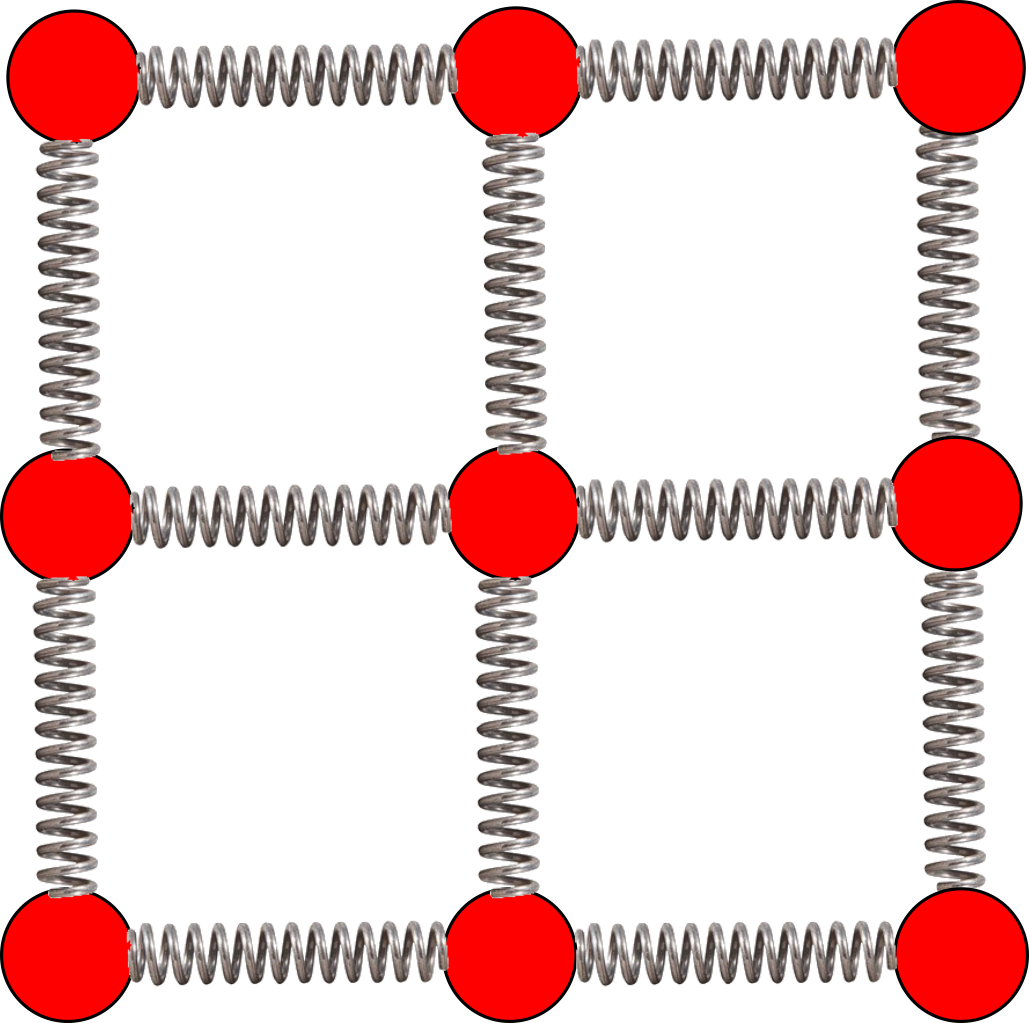
\includegraphics[width=.3\textwidth]{./krystallmodell}
	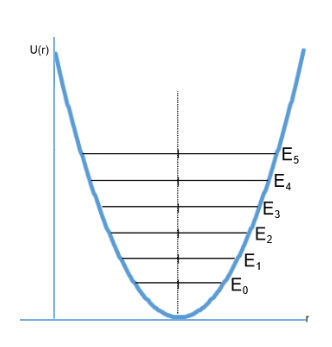
\includegraphics[width=.4\textwidth]{./harmonisk}
	\end{center}
	\caption{Forenklet modell av en krystall der atomene representeres av kuler/massepunkter og kreftene mellom atomene representeres med fjærer. Grafen til høyre skisserer potensiell 	energi som funksjon av forflytning fra likevektsposisjonen i den enkleste tilnærmingen der fjærkraften er $-kx$ slik som i en ideell fjær. Dette er en for grov forenkling for mange anvendelser, og man må da bruke en mer realistisk potensiell energi som den vist i figur \ref{fig:fastelegemer:LennardJones}}
	\label{fig:fastelegemer:krystall}
\end{figure}

Vi innser at denne konfigurasjonen gir en likevektsposisjon for hvert enkelt atom der summen av krefter som virker på det er lik 0. Hvis atomet flyttes litt bort fra likevektsposisjonen vil det virke krefter på det som trekker det mot likevektsposisjonen. Hvis vi antar at kreftene mellom atomene oppfører seg som ideelle fjærer gir disse kreftene opphav til et harmonisk potensial som vist i figur \ref{fig:fastelegemer:krystall}. Så lenge atomet har energi $> 0$ vil det vibrere om likevektsposisjonen sin med en amplitude som er avhengig av hvor stor energi\footnote{Kvantemekanikken forteller oss at atomet aldri kan ha 0 energi, og at energien bare kan være en av et diskret sett verdier. Dette er ikke viktig for denne diskusjonen, så vi ser ikke mer på det her.} det har---og derfor avhengig av temperaturen. 

I denne modellen ser vi at når temperaturen øker vil atomene kunne bevege seg lengre vekk fra likevektspunktet sitt, men den gjennomsnittlige avstanden mellom atomene forblir den samme. Dette ville ikke gi noen målbar termisk utvidelse, så denne modellen er opplagt ikke riktig. Der modellen feiler er at den modellere potensialet atomet beveger seg i som symmetrisk om likevektsposisjonen. Figur \ref{fig:fastelegemer:LennardJones} viser hvordan den potensielle energien, $U(r)$, avhenger av avstanden til naboatomene, $r$, i en typisk krystall. Av kvantemekaniske årsaker er det kun et diskret sett av energitilstander atomet kan befinne seg i. Ved svært lave temperaturer vil praktisk talt alle atomene i krystallen være i den laveste energitilstanden, $E_0$. Når temperaturen øker vil en del atomer eksiteres opp til høyere energitilstander. Vi ser fra potensialgrafen at da skjer to ting: For det første øker rekkevidden av $r$-verdier atomet kan ha. Det vil si at vibrasjonsamplituden øker. For det andre---og viktigere for vår diskusjon---når atomene går opp til høyere energitilstander øker den gjennomsnittlige avstanden mellom atomene og det er dette som forklarer den termiske utvidelsen.

\begin{figure}[tp]
	\begin{center}
	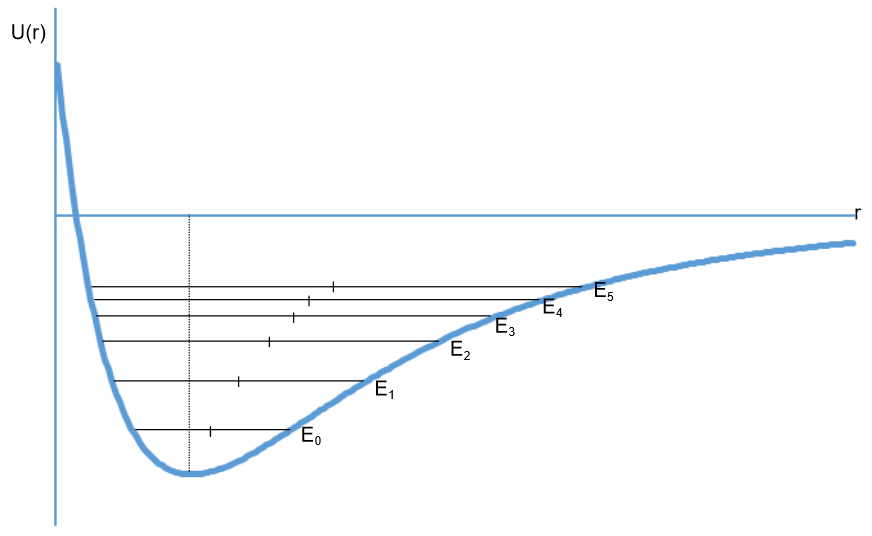
\includegraphics[width=.8\textwidth]{./LennardJones}
	\end{center}
	\caption{Figuren viser et typisk potensial for et atom i en krystall. Av kvantemekaniske årsaker er det kun et diskret sett av energitilstander atomet kan være i. De seks laveste er merket av på figuren som $E_0, E_1, \ldots$. Gjennomsnittlig avstand $r$ til naboatomene er også merket av for hver av de seks energitilstandene.}
	\label{fig:fastelegemer:LennardJones}
\end{figure}

\subsection{Lineær utvidelse}
Makroskopisk viser det seg at termisk utvidelse beskrives godt som direkte proporsjonal med temperaturen. Hvis vi har en stav som ved temperatur $T_0$ har lengde $L_0$ vil den da ved temperatur $T+\Delta T$ ha lengde $L+\Delta L$ der
\begin{equation}
	\Delta L = \alpha L_0\Delta T.
	\label{eq:fastelegemer:deltaL}
\end{equation}
Her er $\alpha$ en koeffisient som er spesifikk for det materialet vi jobber med. Vi ser av ligning (\ref{eq:fastelegemer:deltaL}) at $\alpha$ må ha enhet $\mathrm{K}^{-1}$ (eller $\mathrm{^\circ C}^{-1}$). Typiske verdier av koeffisienten $\alpha$ er av størrelsesorden $10^{-5}~\mathrm{K}^{-1}$.

\subsection{Volumutvidelse}
I tråd med den lineære utvidelsen vi nettopp har sett på vil naturlig nok også volumet av objekter øke når temperaturen øker. Vi skal nå se på volumøkningen av en kube med sidekanter $L_0$. Vi vet at hver sidekant øker lengden fra $L_0$ til $L = L_0+\Delta L$. Dette betyr at volumet øker fra $V_0 = L_0^3$ til $V = (L_0+\Delta L)^3$. Når vi setter inn 	(\label{eq:fastelegemer:deltaL}) finner vi
\begin{displaymath}
\begin{aligned}
	V &= \left[ L_0 + \alpha L_0 \Delta T\right]^3 \\
	&=L_0^3\left[1+\alpha \Delta T\right]^3 \\
	&=V_0 \left[1 + 3\alpha\Delta T + 3(\alpha\Delta T)^2 + (\alpha\Delta T)^3 \right]
\end{aligned}
\end{displaymath}
Siden den termiske utvidelsen for de fleste materialer er svært liten er $\alpha\Delta T\ll1$ for alle realistiske verdier av $\Delta T$. Det betyr at leddene med $(\alpha\Delta T)^2$ og $(\alpha\Delta T)^3$ er av neglisjerbar betydning og vi kan med god presisjon si at 
\begin{displaymath}
	V = V_0(1+3\alpha\Delta T).
\end{displaymath}
Vi ser altså at også den termiske volumutvidelsen til en god tilnærming er direkte proporsjonal med temperaturforskjellen: $V = V_0 + \Delta V$ med
\begin{equation}
	\Delta V = \beta V_0 \Delta T,
\end{equation}
der $\beta = 3\alpha$ er volumutvidelseskoeffisienten.

%\section{Varmekapasitet}

%\section{Varmeledning}

\appendix
\chapter{Maxwellfordelingen}
\label{apx:maxwellfordeling}
Vi skal her utlede Maxwell-fordelingen, altså den fordelingen som beskriver hvilken fart atomene har i en gass med en gitt temperatur. 

Utledning av Maxwell-Boltzmann-statistikk. Fra Kårmund sitt kompendium.

Når vi nå skal utlede hastighetsfordelingen til molekylene i en gass skal vi gjøre to antakelser som forenkler beregningen, og som normalt sett ikke begrenser gyldigheten vesentlig,
\begin{enumerate}
	\item
	Fartsfordelingen er isotropisk; det vil si at det er like stor sannsynlighet for å bevege seg i hvilken som helst retning.
	\item
 	Tettheten er homogen; det vil si at i ethvert volum som er stort nok til at statiske fluktuasjoner i antall gass molekyler kan neglisjeres er tettheten den samme.
\end{enumerate}
Siden sannsynligheten for at et gitt atom har energi $E_i$ er 
\begin{displaymath}
	P(E_i) = \frac{e^{-E_i/kT}}{\sum_j e^{-E_j/kT}}
\end{displaymath}
og siden sammenheng mellom kinetisk energi og hastighet er $E_k = \half m|\vec{v}|^2$, må sannsynlighet for hastighet $\vec{v} = (v_x,v_y,v_z)$ kunne skrives på formen
\begin{displaymath}
	f(\vec{v}) = C\exp\left(-\frac{m|\vec{v}|^2}{2kT}\right) = C\exp\left(-\frac{m}{2kT}\left(v_x^2+v_y^2+v_z^2\right)\right),
\end{displaymath}
der $C$ er en normaliseringskonstant. For å finne $C$ integrerer vi over alle mulige hastigheter, et integral som må ha verdien 1 siden $f(\vec{v})$ beskriver en sannsynlighetsfordeling. Med andre ord må vi ha
\begin{displaymath}
\begin{aligned}
	\frac{1}{C} &= \int_{-\infty}^{\infty}\int_{-\infty}^{\infty}\int_{-\infty}^{\infty}\exp\left(-\frac{m}{2kT}\left(v_x^2+v_y^2+v_z^2\right)\right)\d v_x \d v_y \d v_z \\
	&= \int_{-\infty}^{\infty}\exp\left(-\frac{mv_x^2}{2kT}\right)\d v_x  \int_{-\infty}^{\infty}\exp\left(-\frac{mv_y^2}{2kT}\right)\d v_y  \int_{-\infty}^{\infty}\exp\left(-\frac{mv_z^2}{2kT}\right)\d v_z \\
	&= \left[ \sqrt{\frac{2kT}{m}}\int_{-\infty}^\infty e^{-s^2} \d s\right]^3, 
\end{aligned}
\end{displaymath}
der $s = v_i\sqrt{m/2kT},~i = {x,y,z}$. Det siste integralet er et gaussisk integral, som har løsningen
\begin{displaymath}
	\int_{-\infty}^\infty e^{-s^2} \d s  = \sqrt{\pi}.
\end{displaymath}
Vi finner altså at normaliseringsfaktoren $C$ har verdien
\begin{displaymath}
	C =  \left(\sqrt{\frac{2kT}{m}}\sqrt{\pi}\right)^{-3} = \left(\frac{m}{2\pi kT}\right)^{3/2},
\end{displaymath}
som gir hastighetsfordelingen
\begin{displaymath}
	f(\vec{v}) = \left(\frac{m}{2\pi kT}\right)^{3/2}\exp\left(-\frac{m|\vec{v}|^2}{2kT}\right) 
\end{displaymath}
Hastighetsfordelingen vi har funnet nå er bare et steg på veien til det vi egentlig er interessert i - nemlig fartsfordelingen $f(v)$. Grunnen til at disse to fordelingene er ulike er at det for enhver fart $v$ finnes en rekke kombinasjoner av $v_x, v_y$ og $v_z$ som realiserer denne farten. 

\end{document}